% =====================================================================
%  Analysis map: from raw data to the report (MSP-1, rate-induced tipping)
%  Compiles with pdflatex on Overleaf.
% =====================================================================
\documentclass[11pt]{article}
\usepackage[a4paper,landscape,margin=1.6cm]{geometry}
\usepackage{mathpazo}
\usepackage[T1]{fontenc}
\renewcommand{\ttdefault}{lmtt}
\usepackage{tikz}
\usetikzlibrary{positioning,arrows.meta,fit,calc,backgrounds}
\usepackage{booktabs,tabularx,array}
\usepackage{xcolor}
\usepackage[hidelinks]{hyperref}
\usepackage{enumitem}

\definecolor{accent}{HTML}{7A2E22}
\definecolor{raw}{HTML}{E9E9E9}
\definecolor{ess}{HTML}{F6E7E4}
\definecolor{sup}{HTML}{E4EDF6}
\definecolor{res}{HTML}{FFFFFF}
\definecolor{rep}{HTML}{3A3A3A}

\tikzset{
  base/.style={draw, rounded corners=2pt, align=center, font=\footnotesize, inner sep=4pt, minimum height=0.95cm},
  raw/.style={base, fill=raw, draw=black!45, text width=3.3cm},
  nb/.style={base, fill=ess, draw=accent, line width=0.9pt, text width=3.6cm},
  nbs/.style={base, fill=sup, draw=blue!50!black, dashed, line width=0.9pt, text width=3.6cm},
  res/.style={base, fill=res, draw=black!60, text width=3.3cm},
  rep/.style={base, fill=rep, draw=rep, text=white, text width=3.2cm},
  arr/.style={-{Stealth[length=2.2mm]}, line width=0.7pt, draw=black!70},
  lane/.style={font=\footnotesize\bfseries, text=accent},
}
\usepackage{url}
\makeatletter\g@addto@macro{\UrlBreaks}{\do\_\do-}\makeatother
\newcommand{\nbf}[1]{\nolinkurl{#1}}

\begin{document}

\begin{center}
{\LARGE\bfseries Analysis map: from raw data to the report}\\[4pt]
{\large Rate-induced tipping in a Wien-bridge oscillator}\\[2pt]
Dhruv Kumar Solanki \quad·\quad M.Sc.\ Physics, IIT Bombay \quad·\quad PH 595 M.Sc.\ Project Stage I \quad·\quad guide: Prof.\ P.\ Parmananda
\end{center}

\noindent This document shows, in the order in which the work was done, which notebook of the repository turns which input into which
result, and where each result appears in the report. Notebook files are in \texttt{notebooks/}, inputs in \texttt{data/}, circuits in
\texttt{ltspice/} and \texttt{hardware/}. Every notebook is self-contained: download one, point its INPUTS cell at your files, and run it.

\medskip
\noindent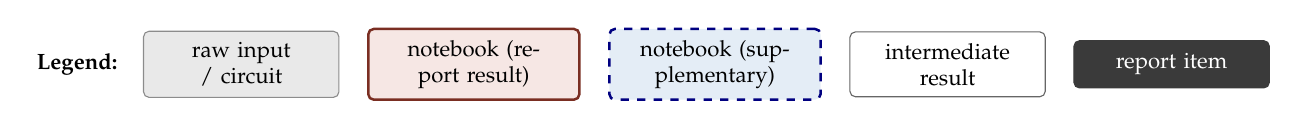
\begin{tikzpicture}[node distance=0.5cm]
  \node[raw, text width=2.2cm, minimum height=0.6cm] (l1) {raw input / circuit};
  \node[nb, text width=2.4cm, minimum height=0.6cm, right=0.35cm of l1] (l2) {notebook (report result)};
  \node[nbs, text width=2.4cm, minimum height=0.6cm, right=0.35cm of l2] (l3) {notebook (supplementary)};
  \node[res, text width=2.2cm, minimum height=0.6cm, right=0.35cm of l3] (l4) {intermediate result};
  \node[rep, text width=2.2cm, minimum height=0.6cm, right=0.35cm of l4] (l5) {report item};
  \node[font=\footnotesize\bfseries, left=0.2cm of l1] {Legend:};
\end{tikzpicture}

\vspace{-2pt}
\begin{center}
\begin{tikzpicture}[node distance=0.45cm and 0.55cm, every node/.append style={text width=2.75cm}]
  % theory
  \node[nb, xshift=3.3cm] (n00) {\nbf{00_theory_numbers}};
  \node[rep, right=0.55cm of n00] (r00) {Ch.~2: Tables 2.2, 2.3; Eqs.\ 2.6, 2.27, 2.33, 2.40, 2.42};
  \node[lane, left=0.35cm of n00, anchor=east, text width=2.3cm, align=right] {Theory (feeds every stage)};
  % stage 1
  \node[raw, below=0.55cm of n00, xshift=0cm] (s1raw) {\texttt{stage1\_ramp/} schematic};
  \node[nb, right=of s1raw] (n01) {\nbf{01_stage1_ltspice_ramp_simulation}};
  \node[nb, right=of n01] (n02) {\nbf{02_stage1_switching_points_and_sqrt_fits}};
  \node[rep, right=of n02] (r1) {Ch.~4: Eqs.\ 4.1--4.3, Figs.\ 4.1, 4.2};
  \node[lane, left=0.35cm of s1raw, anchor=east, text width=2.3cm, align=right] {Stage 1: smooth ramps (simulation)};
  % stage 2
  \node[raw, below=0.55cm of s1raw] (s2raw) {Arduino sketch (A), scope files};
  \node[nb, right=of s2raw] (n03) {\nbf{03_arduino_staircase_and_pot_model}};
  \node[nbs, right=of n03] (n04) {\nbf{04_merge_raw_scope_channels}};
  \node[nb, right=of n04] (n05) {\nbf{05_stage2_switching_points_from_scope}};
  \node[nb, right=of n05] (n06) {\nbf{06_stage2_sqrt_fits_and_hysteresis_loops}};
  \node[rep, below=0.45cm of n06] (r2) {Ch.~5: Eqs.\ 5.1--5.4, Figs.\ 5.1--5.4, Table A.1};
  \node[nbs, below=0.45cm of n05] (n07) {\nbf{07_stage2_cycle_by_cycle_supplementary}};
  \node[lane, left=0.35cm of s2raw, anchor=east, text width=2.3cm, align=right] {Stage 2: the bench, $R_F$ staircase};
  % stage 3
  \node[raw, below=2.0cm of s2raw] (s3raw) {\texttt{stage3\_staircase/} schematic};
  \node[nb, right=of s3raw] (n08) {\nbf{08_stage3_ltspice_staircase_simulation}};
  \node[nb, right=of n08] (n09) {\nbf{09_stage3_simulated_switching_and_min_amplitude}};
  \node[rep, right=of n09] (r3) {Ch.~6: Eqs.\ 6.1--6.3, Figs.\ 6.2, 6.3, Table 6.1};
  \node[lane, left=0.35cm of s3raw, anchor=east, text width=2.3cm, align=right] {Stage 3: the bench in software};
  % stage 4
  \node[raw, below=0.55cm of s3raw] (s4raw) {Arduino sketch (B), bench $R_i$ runs};
  \node[nb, right=of s4raw] (n10) {\nbf{10_stage4_bench_Ri_sweep_tipping}};
  \node[nb, right=of n10] (n11) {\nbf{11_stage4_growth_budget_and_switchoff_law}};
  \node[rep, right=of n11] (r4) {Ch.~7: Table 7.1, Figs.\ 7.1--7.6, Eqs.\ 7.1--7.4};
  \node[raw, below=0.45cm of s4raw] (s4sim) {\texttt{stage4\_Ri/} netlist};
  \node[nb, right=of s4sim] (n12) {\nbf{12_stage4_ltspice_Ri_simulation}};
  \node[nb, right=of n12] (n13) {\nbf{13_stage4_single_sweep_control}};
  \node[rep, right=of n13] (r5) {Ch.~7: Eq.\ 7.5, Figs.\ 7.3b, 7.4, 7.7};
  \node[lane, left=0.35cm of s4raw, anchor=east, text width=2.3cm, align=right] {Stage 4: $R_i$ sweeps, tipping};
  % arrows
  \draw[arr] (n00) -- (r00);
  \draw[arr] (s1raw) -- (n01); \draw[arr] (n01) -- node[above, font=\scriptsize, text width=1cm, align=center]{} (n02); \draw[arr] (n02) -- (r1);
  \draw[arr] (s2raw) -- (n03); \draw[arr] (n03) -- (n04); \draw[arr] (n04) -- (n05); \draw[arr] (n05) -- (n06); \draw[arr] (n06) -- (r2);
  \draw[arr] (n05) -- (n07);
  \draw[arr] (s3raw) -- (n08); \draw[arr] (n08) -- (n09); \draw[arr] (n09) -- (r3);
  \draw[arr] (n05.south east) to[out=-60, in=110] (n09.north);
  \draw[arr] (s4raw) -- (n10); \draw[arr] (n10) -- (n11); \draw[arr] (n11) -- (r4);
  \draw[arr] (s4sim) -- (n12); \draw[arr] (n12) -- (n13); \draw[arr] (n13) -- (r5);
  \draw[arr] (n10.south) -- (n12.north);
\end{tikzpicture}
\end{center}

\noindent\footnotesize The arrow from notebook 05 to 09 means that the simulated runs are analysed with exactly the bench pipeline; the arrow from 10 to
12 means the same for the $R_i$ sweeps. Notebook 03 explains the staircase that notebooks 05, 08, 10 and 12 convert into resistance.
\normalsize

\clearpage
\section*{Stage 1: smooth ramps of $R_F$ in LTspice (report Chapter 4)}
\begin{center}
\begin{tikzpicture}[node distance=0.55cm and 0.75cm]
  \node[raw] (a1) {\nbf{ltspice/stage1_ramp/}\\\nbf{wien_bridge_ramp.asc}\\(R = 1\,k$\Omega$, C = 2\,$\mu$F)};
  \node[raw, below=of a1] (a2) {ramp rates: 36 up from 93.5\,k$\Omega$, 28 down from 100\,k$\Omega$};
  \node[nb, right=of a1, yshift=-0.75cm] (b1) {\nbf{01_stage1_ltspice_ramp_simulation}\\[2pt]\scriptsize runs LTspice; first $|V|>13$ V (on), last $|V|>1.4$ V (off)};
  \node[res, right=of b1, yshift=0.75cm] (c1) {\nbf{time_series_lambda_<rate>.csv}};
  \node[res, below=of c1] (c2) {\nbf{simulation_summary_master.csv}\\(64 switching points)};
  \node[nb, right=of c2] (b2) {\nbf{02_stage1_switching_points_and_sqrt_fits}\\[2pt]\scriptsize $\sqrt{\lambda}$, fixed delay, free exponent; AIC};
  \node[rep, right=of b2, yshift=0.9cm] (d1) {Eqs.\ 4.1, 4.2: $R_{\rm on}$, $R_{\rm off}$ fits};
  \node[rep, below=0.3cm of d1] (d2) {Eq.\ 4.3: $k_{\rm off}=29.4$; $\Lambda_{\rm on}=7.2$};
  \node[rep, below=0.3cm of d2] (d3) {Fig.\ 4.2 (and Fig.\ 4.1 from the time series)};
  \draw[arr] (a1) -- (b1); \draw[arr] (a2) -- (b1); \draw[arr] (b1) -- (c1); \draw[arr] (b1) -- (c2); \draw[arr] (c2) -- (b2);
  \draw[arr] (b2) -- (d1.west); \draw[arr] (b2) -- (d2.west); \draw[arr] (b2) -- (d3.west); 
\end{tikzpicture}
\end{center}

\section*{Stage 2: the bench circuit, staircase of $R_F$ (report Chapters 3 and 5)}
\begin{center}
\begin{tikzpicture}[node distance=0.55cm and 0.6cm]
  \node[raw] (a1) {\nbf{hardware/Rf_sweep_staircase.ino}\\(32 steps up, 32 down)};
  \node[raw, below=of a1] (a2) {oscilloscope: \nbf{TEK000nn.CSV}\\(one file per channel)};
  \node[nb, right=of a1] (b0) {\nbf{03_arduino_staircase_and_pot_model}\\[2pt]\scriptsize taps, mid-step line, true rate};
  \node[nbs, right=of a2] (b1) {\nbf{04_merge_raw_scope_channels}\\[2pt]\scriptsize cut at the trigger pulse};
  \node[res, right=of b1] (c1) {\nbf{newexpdata - <rate>ohms.csv}\\(17 runs)};
  \node[nb, above=of c1] (b2) {\nbf{05_stage2_switching_points_from_scope}\\[2pt]\scriptsize $t_{90}$, $t_{10}$, true $\tau$, $R_{\rm on}$, $R_{\rm off}$};
  \node[res, right=of b2] (c2) {\nbf{Masteranalysis2.csv}\\(one row per cycle)};
  \node[nb, right=of c2, yshift=-0.2cm] (b3) {\nbf{06_stage2_sqrt_fits_and_hysteresis_loops}};
  \node[nbs, below=of b3] (b4) {\nbf{07_stage2_cycle_by_cycle_supplementary}};
  \node[rep, above=0.35cm of b3] (d1) {Eqs.\ 5.1--5.4; $G_c\approx3.07$; Figs.\ 5.2--5.4; Table A.1};
  \node[rep, left=0.6cm of d1] (d0) {Fig.\ 5.1, Fig.\ 3.6};
  \node[rep, below=of b4] (d2) {supplementary checks (Sec.\ 5.2)};
  \node[rep, above=0.35cm of b0] (d3) {Sec.\ 3.2: Eq.\ 3.1, Fig.\ 3.3, Table 3.1};
  \draw[arr] (a1) -- (b0); \draw[arr] (a2) -- (b1); \draw[arr] (b1) -- (c1); \draw[arr] (c1) -- (b2); \draw[arr] (b0) -- (b2);
  \draw[arr] (b2) -- (c2); \draw[arr] (c2) -- (b3); \draw[arr] (c2) |- (b4); \draw[arr] (b3) -- (d1); \draw[arr] (b4) -- (d2); \draw[arr] (b2) -- (d0); \draw[arr] (b0) -- (d3);
\end{tikzpicture}
\end{center}

\clearpage
\section*{Stage 3: the bench staircase simulated (report Chapter 6)}
\begin{center}
\begin{tikzpicture}[node distance=0.55cm and 0.75cm]
  \node[raw] (a1) {\nbf{ltspice/stage3_staircase/}\\\nbf{wien_bridge_staircase.asc}};
  \node[raw, below=of a1] (a2) {43 nominal rates,\\50 $\Omega$/s to 100 k$\Omega$/s};
  \node[nb, right=of a1, yshift=-0.75cm] (b1) {\nbf{08_stage3_ltspice_staircase_simulation}\\[2pt]\scriptsize PWL staircase as the Arduino; LTspice};
  \node[res, right=of b1, yshift=0.75cm] (c1) {\nbf{simdata - <rate>ohms.csv.gz}, \nbf{sim_runlog.csv}};
  \node[nb, right=of c1] (b2) {\nbf{09_stage3_simulated_switching_and_min_amplitude}\\[2pt]\scriptsize bench pipeline of notebook 05, exact $\tau$};
  \node[res, below=of b2] (c2) {\nbf{Masteranalysis_SIM.csv}};
  \node[rep, right=of b2, yshift=0.6cm] (d1) {Eqs.\ 6.1, 6.2; Table 6.1; Fig.\ 6.2};
  \node[rep, below=0.3cm of d1] (d2) {Eq.\ 6.3: $\lambda_c^{\rm (on)}$; Fig.\ 6.3 ($A_{\min}=e^{-\Gamma_-}$)};
  \draw[arr] (a1) -- (b1); \draw[arr] (a2) -- (b1); \draw[arr] (b1) -- (c1); \draw[arr] (c1) -- (b2); \draw[arr] (b2) -- (c2); \draw[arr] (c2) -| (d2.south);
  \draw[arr] (b2) -- (d1.west); \draw[arr] (b2) -- (d2.west);
\end{tikzpicture}
\end{center}

\section*{Stage 4: sweeps of $R_i$ and rate-induced tipping (report Chapter 7)}
\begin{center}
\begin{tikzpicture}[node distance=0.5cm and 0.6cm]
  \node[raw] (a1) {\nbf{hardware/Ri_sweep_staircase.ino}\\(32-step hold, then up/down)};
  \node[raw, below=of a1] (a2) {19 bench runs,\\\nbf{time_series_cropped_<delay>a.csv}};
  \node[nb, right=of a2] (b1) {\nbf{10_stage4_bench_Ri_sweep_tipping}\\[2pt]\scriptsize cycle peaks, state, first switch-off};
  \node[res, right=of b1] (c1) {\nbf{bench_runs.csv}, \nbf{bench_cycles.csv}};
  \node[nb, right=of c1] (b2) {\nbf{11_stage4_growth_budget_and_switchoff_law}\\[2pt]\scriptsize $\sqrt{\lambda}$ / exact law, $G_c$, $\Gamma_+$, $\delta$};
  \node[rep, above=0.4cm of b1] (d1) {Table 7.1; Figs.\ 7.1--7.4; Eq.\ 7.1: $6.06<\lambda_c<6.20$ k$\Omega$/s};
  \node[rep, above=0.4cm of b2] (d2) {Eqs.\ 7.2--7.4: $G_c=3.081$, $\Gamma_+\approx11$; Figs.\ 7.5, 7.6};
  \node[raw, below=1.1cm of a2] (a3) {\nbf{ltspice/stage4_Ri/}\\netlist; 31 step times; 26 single sweeps};
  \node[nb, right=of a3] (b3) {\nbf{12_stage4_ltspice_Ri_simulation}\\[2pt]\scriptsize same pipeline, exact $\tau$};
  \node[res, right=of b3] (c3) {\nbf{sim_runs.csv}, \nbf{sim_cycles.csv}};
  \node[nb, below=of b3] (b4) {\nbf{13_stage4_single_sweep_control}\\[2pt]\scriptsize tanh step, Eq.\ 2.13 along the path};
  \node[res, right=of b4] (c4) {\nbf{single_sweep_summary.csv}};
  \node[rep, right=of c3] (d3) {Eq.\ 7.5: $21.5<\lambda_c^{\rm sim}<32.3$ k$\Omega$/s; Figs.\ 7.3b, 7.4};
  \node[rep, right=of c4] (d4) {Sec.\ 7.7, Fig.\ 7.7};
  \draw[arr] (a1) -- (b1.north west); \draw[arr] (a2) -- (b1); \draw[arr] (b1) -- (c1); \draw[arr] (c1) -- (b2); \draw[arr] (b1) -- (d1); \draw[arr] (b2) -- (d2);
  \draw[arr] (a3) -- (b3); \draw[arr] (b3) -- (c3); \draw[arr] (c3) -- (d3); \draw[arr] (a3) |- (b4); \draw[arr] (b4) -- (c4); \draw[arr] (c4) -- (d4);
  \draw[arr] (b1) -- (b3);
\end{tikzpicture}
\end{center}

\clearpage
\section*{Every notebook}
\footnotesize
\renewcommand{\arraystretch}{1.3}
\begin{tabularx}{\linewidth}{@{}c>{\raggedright\arraybackslash}p{5.2cm}>{\raggedright\arraybackslash}X>{\raggedright\arraybackslash}X>{\raggedright\arraybackslash}p{4.3cm}c@{}}
\toprule
\textbf{Order} & \textbf{Notebook} & \textbf{Inputs (sample in \texttt{data/})} & \textbf{Outputs} & \textbf{Report items} & \textbf{Type} \\
\midrule
0 & \nbf{00_theory_numbers} & component values & Tables 2.2, 2.3 (CSV); budget plot & Ch.~2: Eqs.\ 2.6, 2.27, 2.33, 2.40, 2.42; Tables 2.2, 2.3 & report \\
1 & \nbf{01_stage1_ltspice_ramp_simulation} & Stage 1 schematic; rates (LTspice) or saved time series & time series; switching points & Sec.\ 4.1, Fig.\ 4.1 & report \\
2 & \nbf{02_stage1_switching_points_and_sqrt_fits} & \texttt{simulation\_summary\_master.csv} & fits, exponents, $k_{\rm off}$, $\Lambda_{\rm on}$ & Eqs.\ 4.1--4.3, Fig.\ 4.2 & report \\
3 & \nbf{03_arduino_staircase_and_pot_model} & step delay, circuit values & staircase plots, rate tables & Eq.\ 3.1, Fig.\ 3.3, Table 3.1, Sec.\ 3.5 & report \\
4 & \nbf{04_merge_raw_scope_channels} & two Tektronix channel files & three-column run file & Sec.\ 3.3 (how the files were made) & supplementary \\
5 & \nbf{05_stage2_switching_points_from_scope} & three-column run file(s) & per-cycle $R_{\rm on}$, $R_{\rm off}$; master table; check plots & Sec.\ 5.2, Fig.\ 5.1, Table A.1 & report \\
6 & \nbf{06_stage2_sqrt_fits_and_hysteresis_loops} & \texttt{Masteranalysis2.csv}; raw runs for loops & fits, AIC, $G_c$, first critical rate, loops & Eqs.\ 5.1--5.4, Figs.\ 5.2--5.4, Table A.1 & report \\
7 & \nbf{07_stage2_cycle_by_cycle_supplementary} & master table; raw runs & $V_{\rm out}$ against $R_F$ per cycle; lag per cycle & checks for Sec.\ 5.2 & supplementary \\
8 & \nbf{08_stage3_ltspice_staircase_simulation} & Stage 3 schematic; rates (LTspice) & simulated runs, PWL files, run log & Sec.\ 6.1 & report \\
9 & \nbf{09_stage3_simulated_switching_and_min_amplitude} & one simulated run; \texttt{Masteranalysis\_SIM.csv} & fits, Table 6.1, $A_{\min}$, $\lambda_c^{\rm (on)}$ & Eqs.\ 6.1--6.3, Figs.\ 6.2, 6.3, Table 6.1 & report \\
10 & \nbf{10_stage4_bench_Ri_sweep_tipping} & bench $R_i$ runs & run and cycle tables; cycle map; tipping diagram & Table 7.1, Figs.\ 7.1--7.4, Eq.\ 7.1 & report \\
11 & \nbf{11_stage4_growth_budget_and_switchoff_law} & \texttt{bench\_runs.csv} & switch-off fits, $G_c$, $\Gamma_+$, $\delta$ & Eqs.\ 7.2--7.4, Figs.\ 7.5, 7.6 & report \\
12 & \nbf{12_stage4_ltspice_Ri_simulation} & netlist; step times (LTspice) or simulated runs & simulated run and cycle tables & Eq.\ 7.5, Figs.\ 7.3b, 7.4 & report \\
13 & \nbf{13_stage4_single_sweep_control} & netlist; rates (LTspice) or simulated single sweeps & switching points, final states, prediction & Sec.\ 7.7, Fig.\ 7.7 & report \\
\bottomrule
\end{tabularx}

\normalsize
\medskip
\noindent Notebooks 01, 08, 12 and 13 need LTspice only for their simulation cells (switched off by default); all analysis cells run on
the included samples. Each notebook ends with a check cell that compares its output with the numbers printed in the report.
\end{document}
